\documentclass[12pt, accentcolor=tud9c, linedtoc, bigchapter, colorback, noresetcounter, numbersubsubsec]{tudreport}
\usepackage[utf8]{inputenc}
\usepackage{nomencl}
\usepackage{amsmath}
\usepackage{listings}
\usepackage{hyphenat}
\usepackage{hyperref}
\usepackage{enumerate}
\date{\today}

\title{WS2012/2013 Implementation of Programming Languages}

\subtitle{Reshapes - Drawing Application using EScala library}

\institution{TU Darmstadt\\Software Technology Group}

\begin{document}

\maketitle
\tableofcontents

\chapter{Introduction}

\section{Task}

\section{EScala Tutorial?}

\chapter{Application features and manual}

\section{Add new tabs}

After starting the application the window looks like this: \\
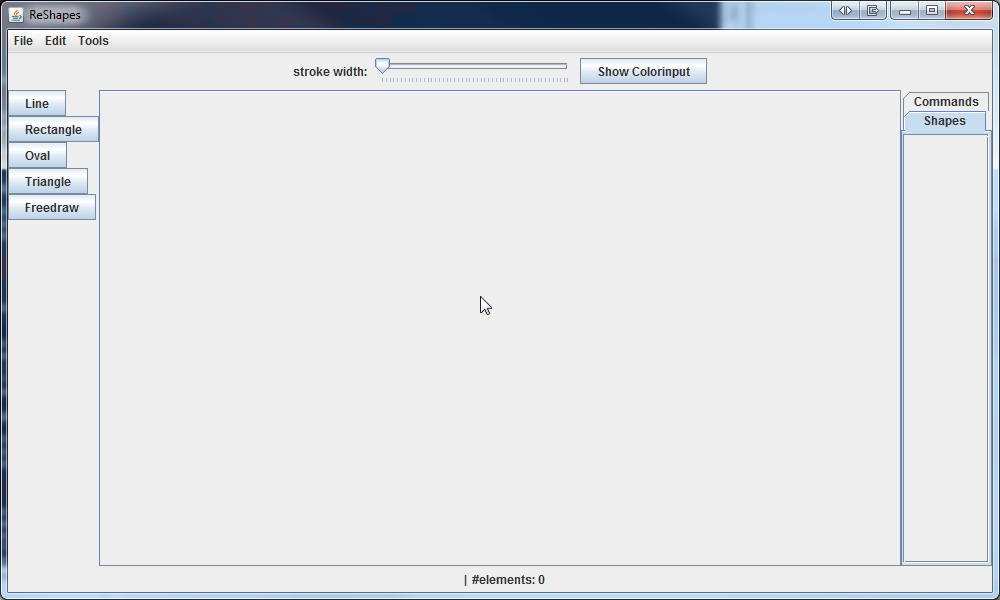
\includegraphics[width=1\textwidth]{img/startup_window} \\

To start drawing you have to add tab with \textbf{File $\rightarrow$ New Tab} \\
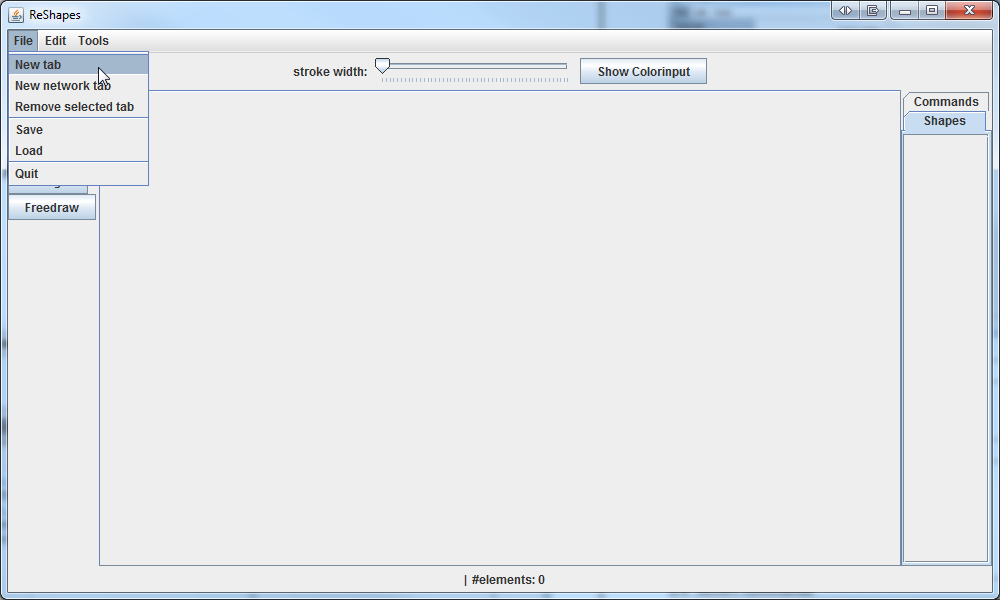
\includegraphics[width=1\textwidth]{img/add_new_tab_1} \\
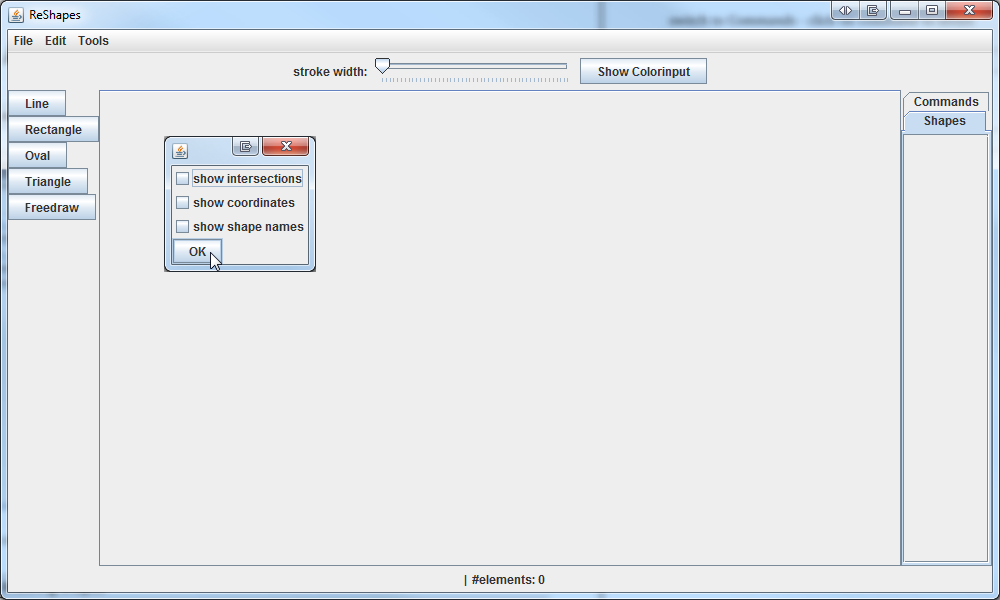
\includegraphics[width=1\textwidth]{img/add_new_tab_2} 

The presented options in the dialog modifiy the drawing space:
\begin{itemize}
    \item \textbf{show intersections:} 
        Displays a small red circle on the intersection point of two shapes
    \item \textbf{show coordinates:}
        Draws a coordinate system instead of the plain white background
    \item \textbf{show shape names:}
        Writes the name of each drawn shape besides it
\end{itemize}

After pressing \textbf{OK} a new tab appears. \\
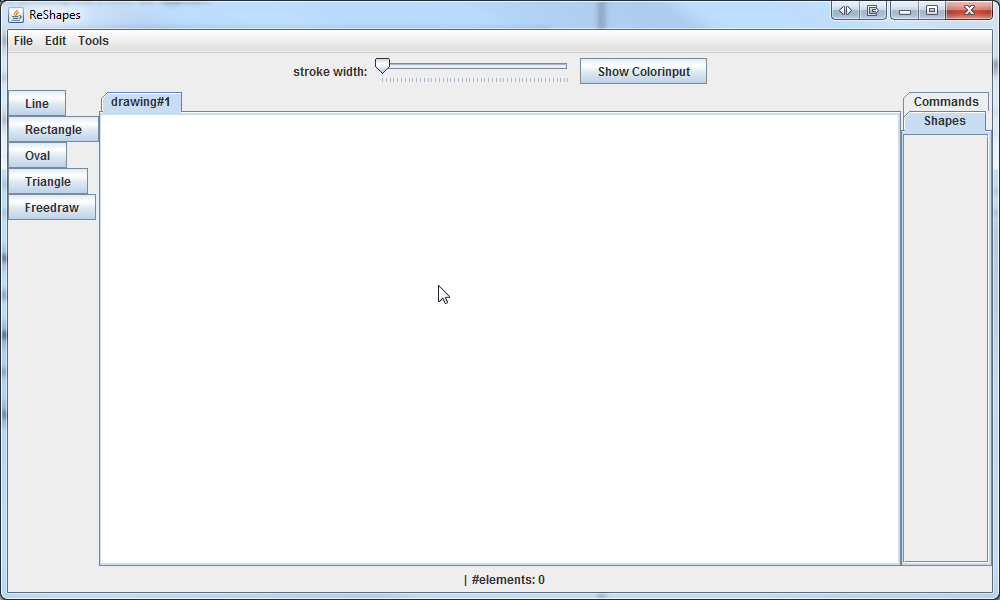
\includegraphics[width=1\textwidth]{img/add_new_tab_3} 

\section{Drawing shapes}

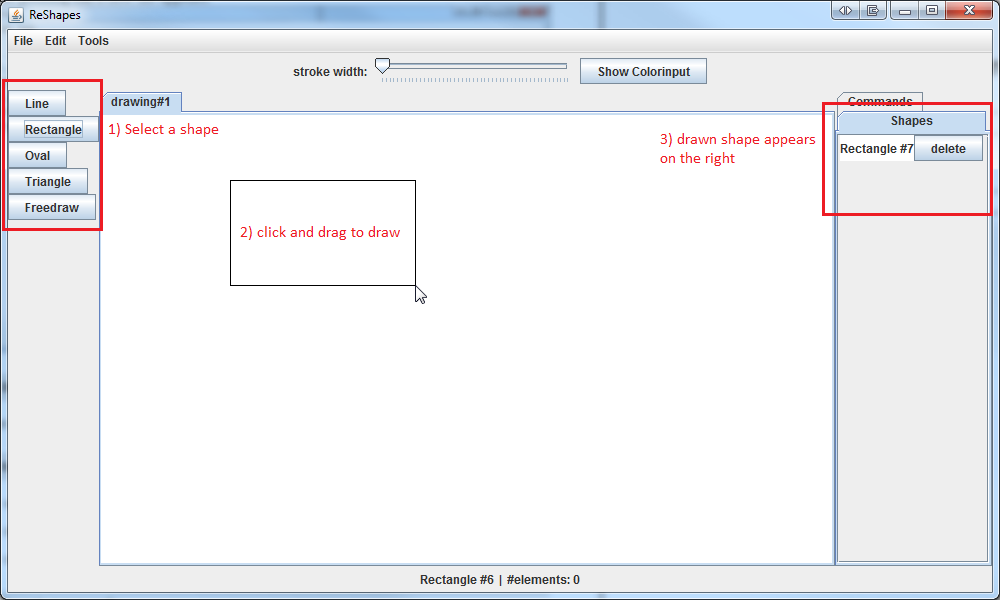
\includegraphics[width=1\textwidth]{img/drawing_shape}

\section{Edit drawn shapes}

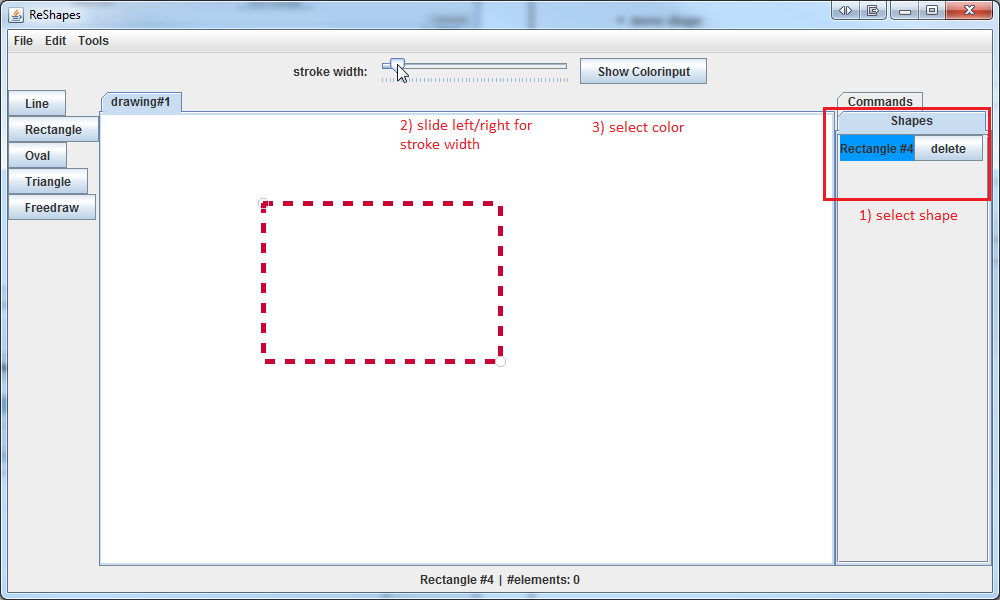
\includegraphics[width=1\textwidth]{img/set_stroke} \\
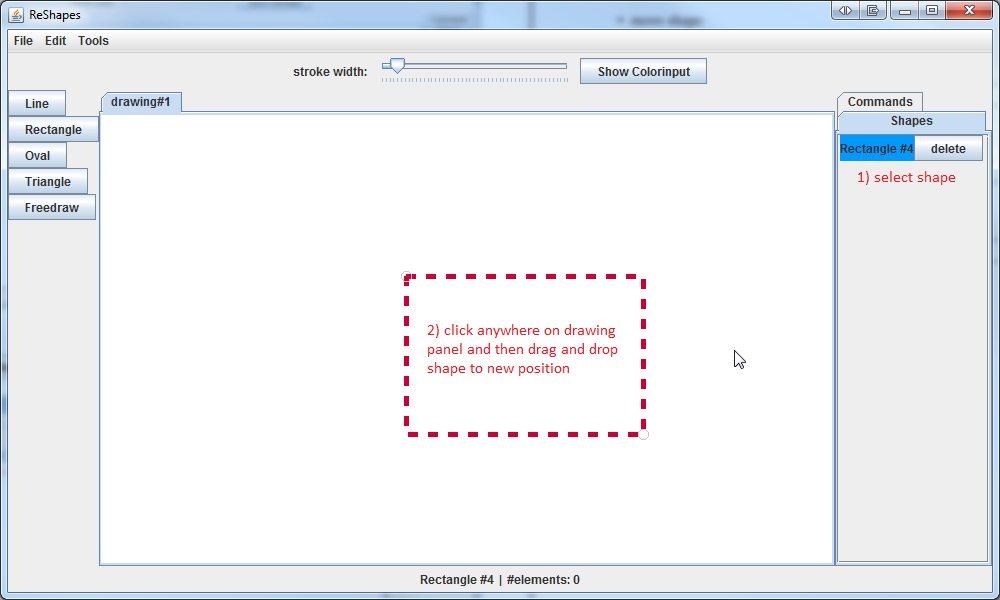
\includegraphics[width=1\textwidth]{img/move_shape} \\
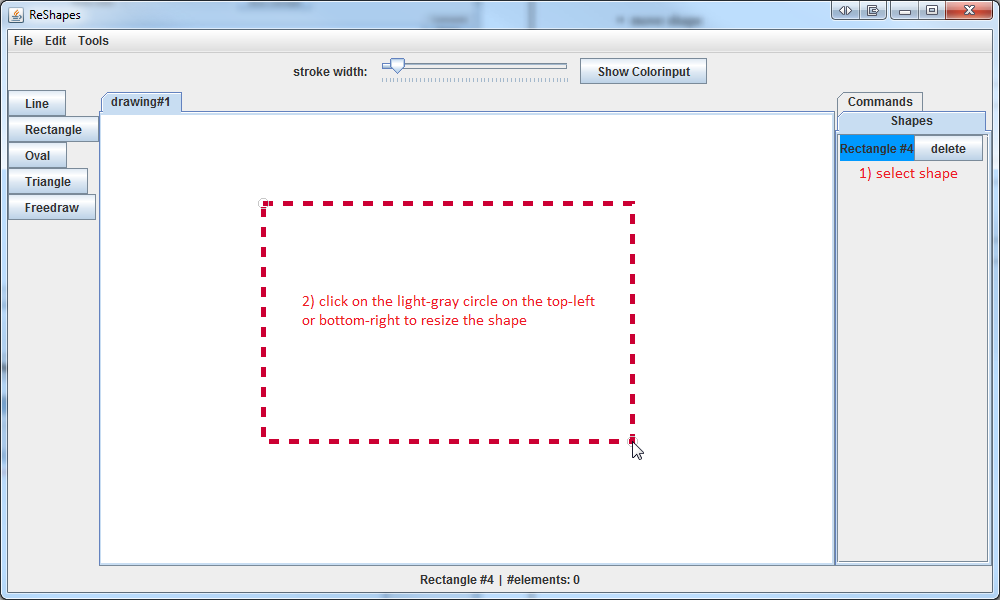
\includegraphics[width=1\textwidth]{img/resize_shape}

\section{Revert commands}

switch to Commands - click on command to revert


\section{Merge tabs}

select tab - click Tools->merge with\dots

\section{Save and Load}

\chapter{Application architecture}

\section{General architecture}
UML, \dots

\section{Uses of EScala library}

\chapter{Possible Refactoring and Enhancements}

\section{Refactoring}

\section{Enhancements}

\end{document}


